\section{شبیه‌سازی استند سه درجه آزادی در محیط سیمولینک}\label{quadall3}
در این بخش به بررسی و شبیه‌سازی مدل دینامیکی استند سه درجه آزادی پرداخته شده است. در بخش \ref{spacestate} فرم فضای حالت استند چهارپره استخراج شد. در شبیه‌سازی نیز از همین روابط استخراج شده، استفاده شده است. مدل شبیه‌سازی شده از استند (شکل \ref{quadsimulink}) دارای چهار ورودی سرعت دورانی موتورها  و دارای سه خروجی زوایای رول ($\phi$)، پیچ ($\theta$)، یاو ($\psi$) و  سه سرعت زاویه‌ای
 ,p
q
 و 
r 
 است.
 
 
\begin{figure}[H]
	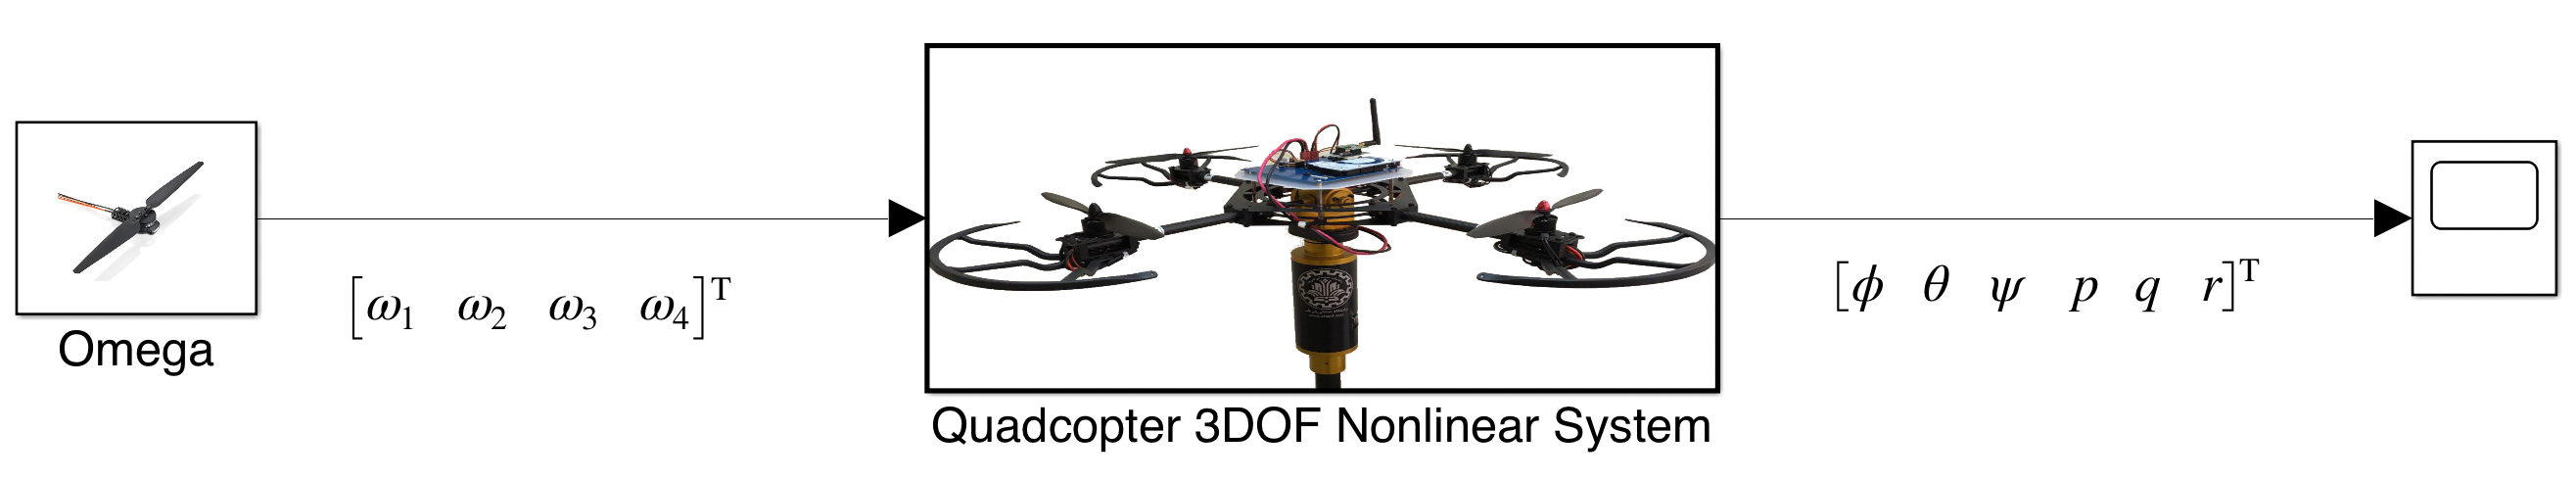
\includegraphics[width=16cm]{../../Figures/QuadSimulation/Stand_Model.png}
	\centering
	\vspace*{-15mm}
	\caption{مدل استند چهارپره شبیه‌سازی شده در سیمولینک و نمایش ورودی و خروجی‌های مدل}
	\label{quadsimulink}
\end{figure}
نمایی از داخل بلوک
\lr{Quacopter 3DOF Nonlinear System}
در شکل \ref{Quad3DOF} آورده شده است.
%\newline
%\newline
\begin{figure}[H]
	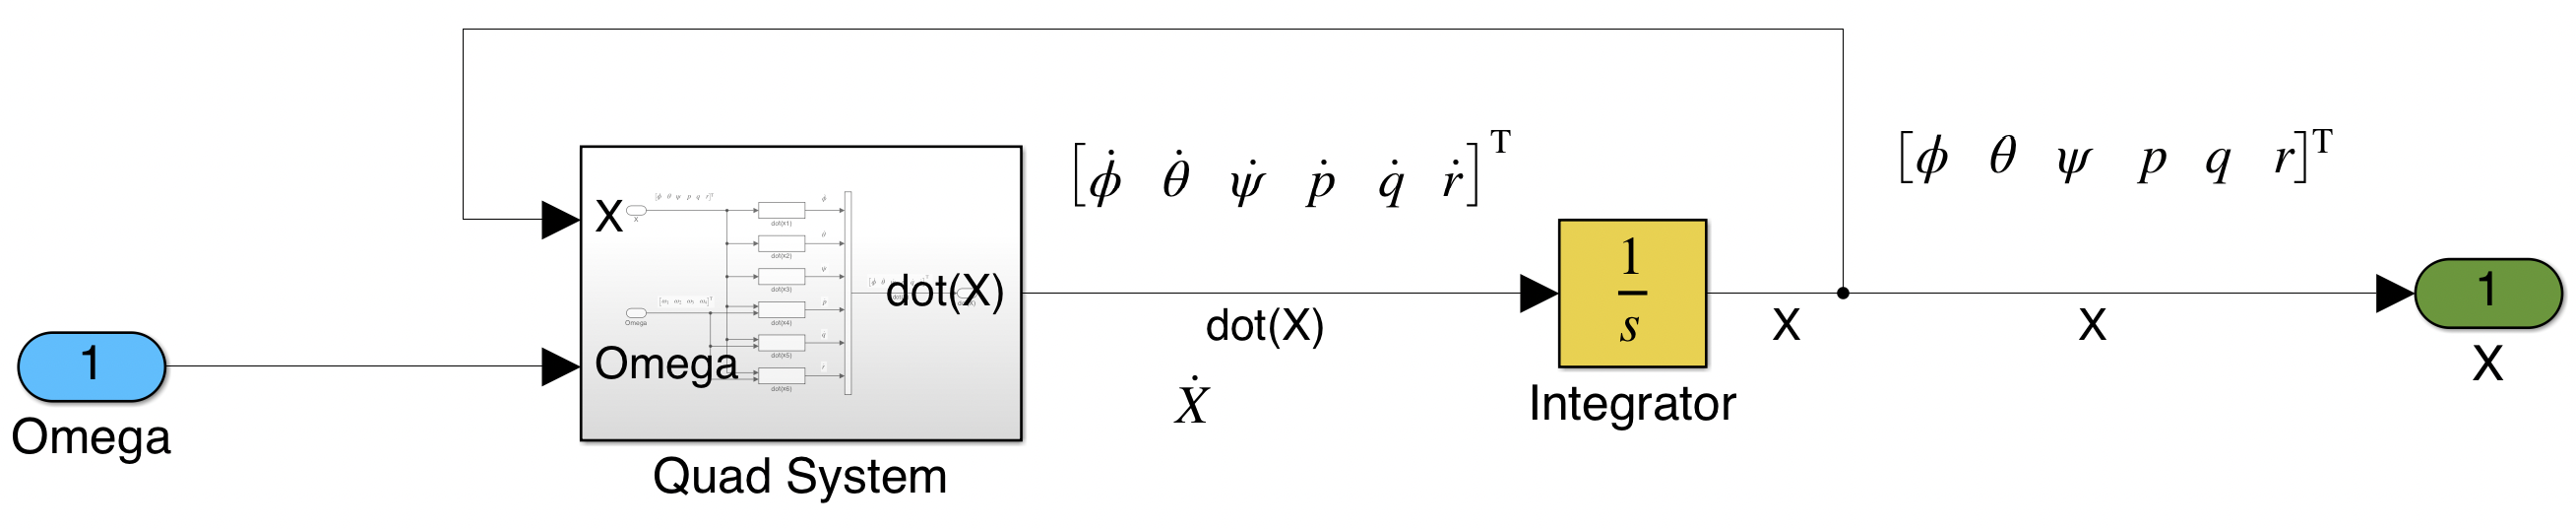
\includegraphics[width=16cm]{../../Figures/QuadSimulation/Integrator.png}
	\centering
	\vspace*{-15mm}
	\caption{مدل استند چهارپره شبیه‌سازی شده در سیمولینک و نمایش ورودی و خروجی‌های مدل}
	\label{Quad3DOF}
\end{figure}
خروجی بلوک
\lr{Quad System}،
$\dot X$
است. با استفاده از بلوک انتگرال‌گیر (بلوک زرد رنگ در شکل \ref{Quad3DOF})
از خروجی بلوک بر اساس شرایط اولیه استند انتگرال گرفته می‌شود و وضعیت استند (زاویه‌های رول ($\phi$)، پیچ ($\theta$)، یاو ($\psi$) و سرعت‌های زاویه‌ای‌
,p
q
و 
(r
را خروجی می‌دهد.

در داخل بلوک
\lr{Quad System}،
شش بلوک دیگر قرار دارد که تعدادی از آن‌ها دارای ورودی $X$ و تعدادی دیگر دارای ورودی $X$ و $\omega$ هستند. مجموع خروجی این شش بلوک $\dot X$ است که در توضیحات بلوک
\lr{Quad System}،
 نیز به آن اشاره شد.
نمایی از داخل بلوک
\lr{Quad System}
در شکل \ref{all-six} آورده شده است.
\begin{figure}[H]
	\includegraphics[width=16cm]{../../Figures/QuadSimulation/all-six.png}
	\centering
%	\vspace*{-15mm}
	\caption{نمایی از داخل بلوک \lr{Quad System}}
	\label{all-six}
\end{figure}